\documentclass{article}

\setlength{\headsep}{0.75 in}
\setlength{\parindent}{0 in}
\setlength{\parskip}{0.1 in}

%=====================================================
% Add PACKAGES Here (You typically would not need to):
%=====================================================

\usepackage{xcolor}
\usepackage[margin=1in]{geometry}
\usepackage{amsmath,amsthm}
\usepackage{fancyhdr}
\usepackage{enumitem}
\usepackage{graphicx}
\usepackage{amsmath, amssymb}  % Include the amsmath and amssymb packages for mathematical symbols

%=====================================================
% Ignore This Part (But Do NOT Delete It:)
%=====================================================

\theoremstyle{definition}
\newtheorem{problem}{Problem}
\newtheorem*{fun}{Fun with Algorithms}
\newtheorem*{challenge}{Challenge Yourself}
\def\fline{\rule{0.75\linewidth}{0.5pt}}
\newcommand{\finishline}{\begin{center}\fline\end{center}}
\newtheorem*{solution*}{Solution}
\newenvironment{solution}{\begin{solution*}}{{\finishline} \end{solution*}}
\newcommand{\grade}[1]{\hfill{\textbf{($\mathbf{#1}$ points)}}}
\newcommand{\thisdate}{April 25, 2024}
\newcommand{\thissemester}{\textbf{Rutgers: Spring 2024}}
\newcommand{\thiscourse}{ECE 509: Convex Optimization} 
\newcommand{\thishomework}{Number} 
\newcommand{\thisname}{Name} 
\newcommand{\thisextension}{Yes/No} 

\headheight 40pt              
\headsep 10pt
\renewcommand{\headrulewidth}{0pt}
\pagestyle{fancy}

\newcommand{\thisheading}{
   \noindent
   \begin{center}
   \framebox{
      \vbox{\vspace{2mm}
    \hbox to 6.28in { \textbf{\thiscourse \hfill \thissemester} }
       \vspace{4mm}
       \hbox to 6.28in { {\Large \hfill Homework \#\thishomework \hfill} }
       \vspace{2mm}
         \hbox to 6.28in { { \hfill \thisdate  \hfill} }
       \vspace{2mm}
       \hbox to 6.28in { \emph{Name: \thisname \hfill Extension: \thisextension}}
      \vspace{2mm}}
      }
   \end{center}
   \bigskip
}

%=====================================================
% Some useful MACROS (you can define your own in the same exact way also)
%=====================================================


\newcommand{\ceil}[1]{{\left\lceil{#1}\right\rceil}}
\newcommand{\floor}[1]{{\left\lfloor{#1}\right\rfloor}}
\newcommand{\prob}[1]{\Pr\paren{#1}}
\newcommand{\expect}[1]{\Exp\bracket{#1}}
\newcommand{\var}[1]{\textnormal{Var}\bracket{#1}}
\newcommand{\set}[1]{\ensuremath{\left\{ #1 \right\}}}
\newcommand{\poly}{\mbox{\rm poly}}


%=====================================================
% Fill Out This Part With Your Own Information:
%=====================================================


\renewcommand{\thishomework}{8} %Homework number
\renewcommand{\thisname}{Ravi Raghavan} % Enter your name here
\renewcommand{\thisextension}{No} % Pick only one of the two options accordingly

\begin{document}

\thisheading
\vspace{-0.75cm}


%=====================================================
% LaTeX Tip: You can erase this part from here.... 
%=====================================================		

\finishline

%=====================================================
% LaTeX Tip: ... to here
%=====================================================	


\bigskip
\begin{problem} Problem 3.20
\textit{Composition with an affine function.} Show that the following function $f: \mathbb{R}^n \rightarrow \mathbb{R}$ are convex
\begin{itemize}
    \item[(a)] $f(x) = ||Ax - b||$, where $A \in \mathbb{R}^{m x n}$, $b \in \mathbb{R}^m$, and $||.||$ is a norm on $\mathbb{R}^m$
    \begin{solution}
    Let us have $x, y \in dom f$. Our goal is, for $\theta \in [0, 1]$ to prove that $f(\theta x + (1 - \theta) y ) \leq \theta f(x) + (1 - \theta) f(y)$

    $f(\theta x + (1 - \theta) y ) = ||A(\theta x + (1 - \theta) y) - b|| = ||\theta 
 Ax + (1 - \theta) Ay - b||$

The triangle inequality theorem(i.e. $||x|| + ||y|| \geq ||x + y||$) also states that: \newline 
$\theta f(x) + (1 - \theta) f(y) = \theta ||Ax - b|| + (1 - \theta) ||Ay - b|| =  ||\theta(Ax - b)|| + ||(1 - \theta)(Ay - b)|| \geq ||\theta (Ax - b) + (1 - \theta) (Ay - b)|| = ||\theta Ax - \theta b + (1 - \theta) Ay -  (1 - \theta)b|| = ||\theta Ax  + (1 - \theta) Ay - b|| = f(\theta x + (1 - \theta) y )$ \newline 

Another way of doing this proof is just by seeing that $f(x)$ is a composition of a norm and an affine function. Norms are convex. Hence, since we have a composition with an affine mapping, we have a convex function! 
 
    \end{solution} 

    \item[(b)] $f(x) = - (\det (A_0 + x_1 A_1 + \dots + x_n A_n))^{\frac{1}{m}}$, on $\{x | A_0 + x_1 A_1 + \dots + x_n A_n \succ 0\}$ where $A_i \in \mathbb{S}^m$

    \begin{solution}
        Let $\lambda_{ij}$ represent the $j$th Eigenvalue of $A_i$. \newline 

        Since $A_i \in \mathbb{S}^m$, the eigenvalues of $A_0 + x_1 A_1 + \dots + x_n A_n$ are just the sum of the individual eigenvalues of $A_0, x_1 A_1, \dots x_n A_n$

        We already know that the determinant of a Symmetric Matrix is the product of its eigenvalues. Hence, we can re-express $f(x)$ as follows: \newline 

        $f(x) = - ((\lambda_{01} + x_1 \lambda_{11} + \dots + x_n \lambda_{n1}) \dots (\lambda_{0m} + x_1 \lambda_{1m} + \dots + x_n \lambda_{nm}))^{\frac{1}{m}}$

        Since $A_0 + x_1 A_1 + \dots + x_n A_n \succ 0$, we know that $(\lambda_{0j} + x_1 \lambda_{1j} + \dots + x_n \lambda_{nj}) > 0$

Hence, we can clearly rewrite our problem: \newline 

        Let us denote $P = \begin{bmatrix}
    \lambda_{11} & \cdots & \lambda_{n1} \\
    \lambda_{12} & \cdots & \lambda_{n2} \\
    \vdots & \ddots & \vdots \\
    \lambda_{1m} & \cdots & \lambda_{nm}
\end{bmatrix}$

Let $Q = \begin{bmatrix}
    \lambda_{01} \\
    \lambda_{02} \\
    \vdots \\
    \lambda_{0m}
\end{bmatrix}$

Let $h(x) = - (\prod_{i=1}^{m} x_i)^{\frac{1}{m}}$ where $x \in \mathbb{R}^m_{++}$ \newline 

Let $g(x) = Px + Q$

$f(x) = h(g(x))$ \newline 

Since geometric means are concave as we proved in class where the domain is $\mathbb{R}^m_{++}$, $h(x)$ is convex. Furthermore, when the domain is $\mathbb{R}^m_{++}$, it is clear that $h(x)$ is non-increasing in each argument. 

$g(x)$ is an affine transformation is, thus, convex and concave. 
        
Hence, we have a case where $h(x)$ is convex and non-increasing and $g(x)$ is concave. This means that $f(x) = h(g(x))$ is Convex. 

As shown, we have shown that $f$ is a Composition of a Convex Function and an Affine Mapping, hence telling us that $f$ is Convex
    \end{solution}
\end{itemize}
\end{problem}

\begin{problem} Problem 3.21
    {Pointwise maximum and supremum.} Show that the following function $f: \mathbb{R}^n \rightarrow \mathbb{R}$ are convex

    \begin{itemize}
        \item[(a)] $f(x) = \max_{i = 1, \dots, k} || A^{(i)}x - b^{(i)}||$, where $A^{(i)} \in \mathbb{R}^{m x n}$, $b^{(i)} \in \mathbb{R}^m$, and $||.||$ is a norm on $\mathbb{R}^m$

        \begin{solution}
            This function is just a pointwise maximum of a bunch of convex functions(this was proved earlier), which are convex. Hence, $f$ is convex. 
        \end{solution}

        \item[(b)] $f(x) = \sum_{i=1}^{r} |x|_{[i]}$ on $\mathbb{R}^n$, where $|x|$ denotes the vector with $|x|_i = |x_i|$ (i.e. $|x|$ is the absolute value $x$, component wise), and $|x|_{[i]}$ is the $i$th largest component of $|x|$.  In other words,  $|x|_{[1]}, |x|_{[2]}, \dots , |x|_{[n]}$ are the absolute values of the components of $x$, sorted in nonincreasing order.

        \begin{solution}
            We can re-express $f(x)$: \newline 

            $f(x) = \max_{i_1, i_2, \dots, i_r} \{|x_{i_1}| + |x_{i_2}| + \dots + |x_{i_r}|\}$ where $i_k \in [1, n] \enspace \forall k \in [1, r]$ \newline 

            It is clear that $f(x)$ is the pointwise maximum of $\binom{n}{r}$ convex functions. 

            
        \end{solution}
    \end{itemize}
\end{problem}


\begin{problem} Problem 3.22
\textit{Composition rules.} Show that the following functions are convex.

\begin{itemize}
    \item[(a)] $f(x) = -\log(-\log(\sum_{i=1}^{m} e^{a_i^Tx + b_i}))$ on $dom f = \{ x | \sum_{i=1}^{m} e^{a_i^Tx + b_i} < 1\}$. You can use the fact that $\log(\sum_{i=1}^{m} e^{y_i})$ is convex. 

    \begin{solution}
        We can re-express $f(x)$ as follows: \newline 

        $f(x) = h(g(Ax + b))$ where $h(x) = - \log(x)$ and $g(x) = -\log(\sum_{i=1}^{m} e^{y_i})$ and $A$ is a matrix such that each $a_i$ is a row of $A$ and $b$ is a vector such that each $b_i$ is a row of $b$. 

        Let's start by first analyzing $g(Ax + b)$. We know that $g$ is concave. Hence, $g(Ax + b)$ is concave. 

        Since $h(x) = - \log(x)$, $h(x)$ is convex. 

        Since we have $h$ is convex, $\tilde{h}$ is nonincreasing and $g(Ax + b)$ is concave, we have that $f$ is convex. 
    \end{solution}

    \item[(e)] $f(x, t) = -\log(t^p - ||x||^p_p)$ where $p > 1$ and $dom f = \{(x, t) | t > ||x||_p \}$. You can use the fact that $\frac{||x||^p_p}{u^{p - 1}}$ is convex in $(x, u)$ for $u > 0$

    \begin{solution}
        Let's start rewriting $f(x, t)$ \newline 

        $f(x, t) = -\log(t^{p - 1}(t - \frac{||x||^p_p}{t^{p - 1}}))$ \newline 

        $f(x, t) = -\log(t^{p - 1}) - \log((t - \frac{||x||^p_p}{t^{p - 1}}))$

        $f(x, t) = -(p - 1)\log(t) - \log((t - \frac{||x||^p_p}{t^{p - 1}}))$

        The function $-(p - 1)\log(t)$ is convex since $p > 1$(i.e. $p - 1 > 0$) and $-\log(t)$ is convex. \newline 

        Let's look at $- \log((t - \frac{||x||^p_p}{t^{p - 1}}))$. This function is a composition of a non-increasing convex function(i.e. $-\log(x)$) and a concave function(i.e. $(t - \frac{||x||^p_p}{t^{p - 1}})$). 

        Let's briefly explain why $(t - \frac{||x||^p_p}{t^{p - 1}})$ is concave. $\frac{||x||^p_p}{t^{p - 1}}$ is convex. Hence, $-\frac{||x||^p_p}{t^{p - 1}}$ is concave. $t$ can be viewed as an affine map. Hence, $t$ is convex and concave. The sum of 2 concave functions is concave. Hence, $(t + (- \frac{||x||^p_p}{t^{p - 1}})) = (t - \frac{||x||^p_p}{t^{p - 1}})$ is Concave. 

        Hence, $- \log((t - \frac{||x||^p_p}{t^{p - 1}}))$ is convex. 

        Since $-(p - 1)\log(t)$ and $- \log((t - \frac{||x||^p_p}{t^{p - 1}}))$ are both convex, $f(x, t) = -(p - 1)\log(t) - \log((t - \frac{||x||^p_p}{t^{p - 1}}))$ is convex as well since it is the sum of $-(p - 1)\log(t)$ and $- \log((t - \frac{||x||^p_p}{t^{p - 1}}))$
    \end{solution}
\end{itemize}
    
\end{problem}

\begin{problem} Problem 3.23
    \textit{Perspective of a Function.}

    \begin{itemize}
        \item[(a)] Show that for $p > 1$, 
        \begin{equation}
            f(x, t) = \frac{|x_1|^p + \dots + |x_n|^p}{t^{p - 1}} = \frac{||x||_p^p}{t^{p - 1}}
        \end{equation}
        is convex on $\{ (x, t) | t > 0\}$

        \begin{solution}
            $f(x, t)$ is the perspective function of $||x||_p^p$ which is convex. 

            Let's briefly show that $||x||_p^p$ is convex. \newline 
            $g(x) = ||x||_p^p = |x_1|^p + \dots + |x_n|^p$ \newline 

            $\frac{\partial g}{x_k} = p |x_k|^{p - 1} sign(x_k)$

            $\frac{\partial^2 g}{x_k^2} = p(p - 1) |x_k|^{p - 2} > 0$

            $\frac{\partial^2 g}{x_j x_k} =0$ where $j \neq k$

            It is clear that this Hessian is a Diagonal Matrix with all positive entries. Hence, the Hessian is Positive Definite which means that $g(x)$ is convex. 
        \end{solution}
    \end{itemize}
\end{problem}

\begin{problem} Problem 3.26
    \begin{itemize}
        \item[(c)] 
        \begin{solution}
            We are given the following fact: \newline 

            $\prod_{i=n - k + 1}^{n} \lambda_i(X) = \inf \{ \prod_{i=1}^{k} (V^T X V)_{ii} | V \in \mathbb{R}^{n x k}, V^TV = I \}$

            Let's analyze $\prod_{i=1}^{k} (V^T X V)_{ii}$ for a given $V$ where $V^TV = I$ \newline 

            $(V^T X V)_{ii} = v_i^T X v_i$ where $v_i$ is the $i$th column of $V$ \newline 

            We also know that $X$ is Positive Definite. Hence, $(V^T X V)_{ii} > 0$ \newline 

            Hence, 
            $\log(\prod_{i=n - k + 1}^{n} \lambda_i(X)) = \inf \{ \log(\prod_{i=1}^{k} (V^T X V)_{ii}) | V \in \mathbb{R}^{n x k}, V^TV = I \}$ \newline 

            $\sum_{i=n - k + 1}^{n} \log(\lambda_i(X)) = \inf \{ \log(\prod_{i=1}^{k} (V^T X V)_{ii}) | V \in \mathbb{R}^{n x k}, V^TV = I \}$

            Since $X$ is symmetric, we know that $V^TXV$ is symmetric as well. This means that $\log(\prod_{i=1}^{k} (V^T X V)_{ii}) = \log \det(V^T X V)$ which is concave. 

            Hence, $\sum_{i=n - k + 1}^{n} \log(\lambda_i(X)) = \inf \{ \log(\prod_{i=1}^{k} (V^T X V)_{ii}) | V \in \mathbb{R}^{n x k}, V^TV = I \}$ can be re-expressed as follows: \newline 

            $\sum_{i=n - k + 1}^{n} \log(\lambda_i(X)) = \inf \{ \log \det (V^T X V) | V \in \mathbb{R}^{n x k}, V^TV = I \}$

            This is clearly a pointwise infimum of a bunch of concave functions. Hence, we know that $\sum_{i=n - k + 1}^{n} \log(\lambda_i(X))$ is Concave. 




            
        \end{solution}
    \end{itemize}
\end{problem}

\begin{problem} Problem 3.32
    \textit{Products and ratios of convex functions.} In general the product or ratio of two convex functions is not convex. However, there are some results that apply to functions on $\mathbb{R}$. Prove the following.

    \begin{itemize}
        \item[(a)] If $f$ and $g$ are convex, both nondecreasing (or nonincreasing), and positive functions on an interval, then $fg$ is convex.

        \begin{solution}
            Goal: Prove that $f(x) g(x)$ is convex. \newline 

            First Derivative of $f(x) g(x) = f'(x) g(x) + f(x) g'(x)$ \newline 

            Second Derivative of $f(x) g(x) = f''(x) g(x) + f'(x) g'(x) + f'(x) g'(x) + f(x) g''(x) = f''(x) g(x) + 2f'(x)g'(x) + f(x) g''(x)$

            Since $f$ and $g$ are convex, we know can replace $f''(x)$ and $g''(x)$ with $k_{f''}$ and $k_{g''}$ where $k_{f''} \geq 0$ and $k_{g''} \geq 0$

            Since $f$ and $g$ are both positive functions, we can replace $f(x)$ and $g(x)$ with $k_{f}$ and $k_{g}$ where $k_{f} \geq 0$ and $k_{g} \geq 0$

            Let's rewrite our expression for the second derivative \newline 

            $f''(x) g(x) + 2f'(x)g'(x) + f(x) g''(x) = k_{f''} k_{g} + 2f'(x)g'(x) + k_{f} k_{g''}$ \newline 

            If $f$ and $g$ are either both nondecreasing or both non-increasing this means that either $f'(x) \geq 0, g'(x) \geq 0$ or $f'(x) \leq 0, g'(x) \leq 0$. Either way, the product $2f'(x)g'(x) \geq 0$ and we can denote this as $k_2$

            Our expression for the second derivative becomes: \newline 
            $k_{f''} k_{g} + k_2 + k_{f} k_{g''} \geq 0$ \newline

            Breakdown: \newline 
            $k_{f''} k_{g} \geq 0$ \newline 
            $k_2 \geq 0$ \newline 
            $k_{f} k_{g''} \geq 0$ \newline 

            By proving that the second derivative $\geq 0$, we have shown convexity

        \end{solution}
        \item[(b)] If $f, g$ are concave, positive, with one nondecreasing and the other nonincreasing, then $fg$ is concave.

        \begin{solution}
            Goal: Prove that $f(x) g(x)$ is convex. \newline 

            First Derivative of $f(x) g(x) = f'(x) g(x) + f(x) g'(x)$ \newline 

            Second Derivative of $f(x) g(x) = f''(x) g(x) + f'(x) g'(x) + f'(x) g'(x) + f(x) g''(x) = f''(x) g(x) + 2f'(x)g'(x) + f(x) g''(x)$

            Since $f$ and $g$ are concave, we know can replace $f''(x)$ and $g''(x)$ with $k_{f''}$ and $k_{g''}$ where $k_{f''} \leq 0$ and $k_{g''} \leq 0$

            Since $f$ and $g$ are both positive functions, we can replace $f(x)$ and $g(x)$ with $k_{f}$ and $k_{g}$ where $k_{f} \geq 0$ and $k_{g} \geq 0$

            If $f$ and $g$ are have one of them nondecreasing and the other nonincreasing this means that either $f'(x) \geq 0, g'(x) \leq 0$ or $f'(x) \leq 0, g'(x) \geq 0$. Either way, the product $2f'(x)g'(x) \leq 0$ and we can denote this as $k_2$

            Our expression for the second derivative becomes: \newline 
            $k_{f''} k_{g} + k_2 + k_{f} k_{g''} \leq 0$ \newline

            Breakdown: \newline 
            $k_{f''} k_{g} \leq 0$ \newline 
            $k_2 \leq 0$ \newline 
            $k_{f} k_{g''} \leq 0$ \newline 

            By proving that the second derivative $\leq 0$, we have shown concavity
            

        \end{solution}
        \item[(c)] If $f$ is convex, nondecreasing, and positive, and $g$ is concave, nonincreasing, and positive, then $f /g$ is convex.
        \begin{solution}
            Let's look at $1/g$ \newline 

            First Derivative of $1/g$: $\frac{-g'(x)}{(g(x))^2}$ \newline 

            Second Derivative of $1/g$: $\frac{-g''(x)(g(x))^2 + 2g(x) (g'(x))^2}{(g(x))^4}$ \newline 

            Since $g$ is concave, $g''(x)$ is $\leq 0$. Hence, $-g''(x)(g(x))^2$ is $\geq 0$. Since $g$ is positive, $2g(x) (g'(x))^2$ is $\geq 0$. 

            Hence, $\frac{-g''(x)(g(x))^2 + 2g(x) (g'(x))^2}{(g(x))^4} \geq 0$

            $1/g$ is convex, nondecreasing, and positive. \newline 

            Since $f$ and $1/g$ are both convex, nondecreasing, and positive, based on Part $(a)$, $f/g$ is convex as well. 

        \end{solution}
    \end{itemize}
\end{problem}

\begin{problem}
    Problem 4.1. Consider the optimization problem 
    \begin{align*}
\text{minimize} \quad & f_0(x_1, x_2) \\
\text{subject to} \quad & 2x_1 + x_2 \geq 1\\
\quad & x_1 + 3x_2 \geq 1\\
& x_1 \geq 0, \enspace x_2 \geq 0
\end{align*}

Make a sketch of the feasible set. For each of the following objective functions, give the optimal set and the optimal value.

\begin{figure}[h!]
        \centering
        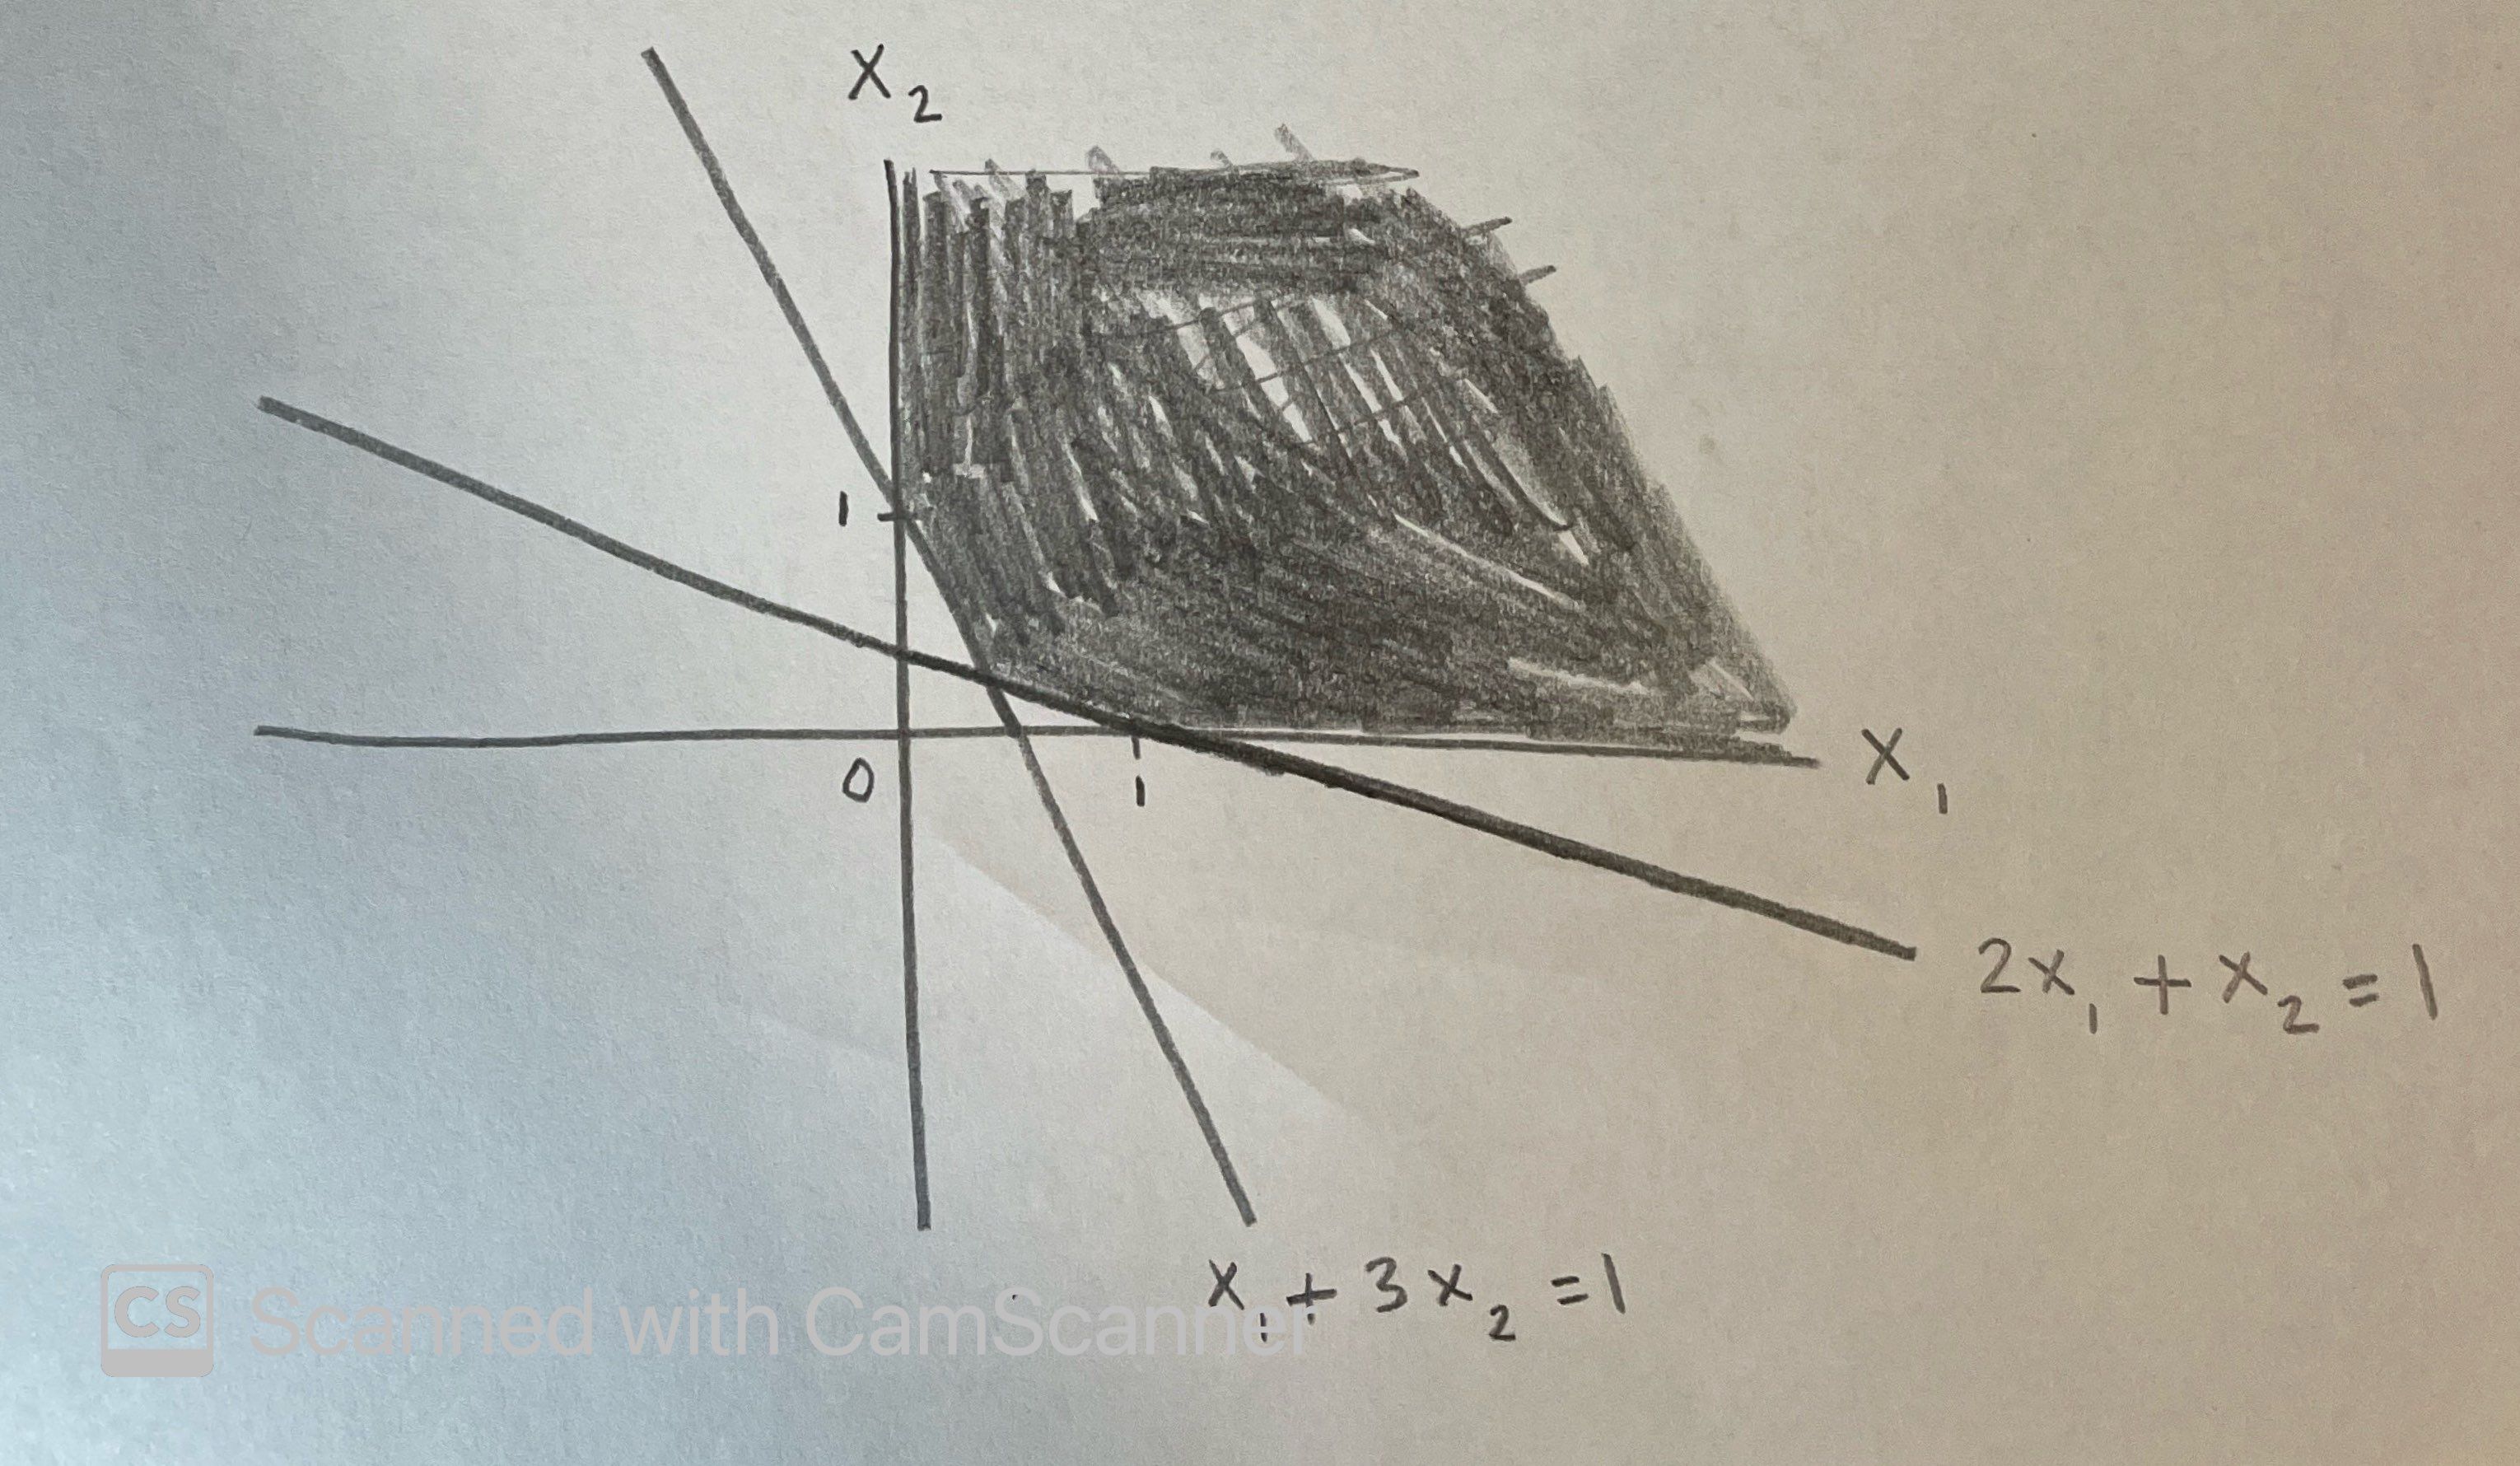
\includegraphics[width=0.6 \textwidth]{HW 8n_1.jpg}
        \caption{Set of Feasible Set}
    \end{figure}

Note: The feasible set is the convex hull of the following points $(0, 1)$, $(0.4, 0.2)$, $(1, 0)$, $(0, \infty)$, $(\infty, 0)$

\begin{itemize}
    \item[(a)] $f_0(x_1, x_2) = x_1 + x_2$
    \begin{solution}
        Optimal Set: $\{(0.4, 0.2)\}$, Optimal Value: $0.6$
    \end{solution}
    \item[(b)] $f_0(x_1, x_2) = - x_1 - x_2$
    \begin{solution}
        This one is unbounded below. Hence, we can essentially say that Optimal Set: $\{(\infty, \infty)\}$, Optimal Value: $-\infty$
    \end{solution}
    \item[(c)] $f_0(x_1, x_2) = x_1$  
    \begin{solution}
        Optimal Set: $\{(0, x_2) | x_2 \geq 1\}$, Optimal Value: $0$
    \end{solution}
    \item[(d)] $f_0(x_1, x_2) = \max\{x_1, x_2\}$
    \begin{solution}
        Optimal Set: $\{(\frac{1}{3}, \frac{1}{3})\}$, Optimal Value: $\frac{1}{3}$
    \end{solution}
    \item[(e)] $f_0(x_1, x_2) = x_1^2 + 9x_2^2$
    \begin{solution}
        Optimal Set: $\{(\frac{1}{2}, \frac{1}{6})\}$, Optimal Value: $0.5$
    \end{solution}
\end{itemize}
\end{problem}

\begin{problem}
    Problem 4.3. Prove that $x^* = (1, \frac{1}{2}, -1)$ is optimal for the optimization problem

    \begin{align*}
\text{minimize} \quad & (1/2)x^TPx + q^Tx + r \\
\text{subject to} \quad & -1 \leq x_i \leq 1, \quad i = 1, 2, 3\\
\end{align*}

where:
\begin{itemize}
    \item $P = \begin{bmatrix}
13 & 12 & -2 \\
12 & 17 & 6 \\
-2 & 6 & 12
\end{bmatrix}$, $q = \begin{bmatrix}
-22.0\\
-14.5\\
13.0
\end{bmatrix}$, $r = 1$
\end{itemize}

\begin{solution}
    The optimality condition is that $\nabla f(x^*) (y - x^*) \geq 0$

    $\nabla f(x) = Px + q$ \newline 
    $\nabla f(x^*) = (-1, 0, 2)$

Substituting this back into the optimality condition means that: \newline 
$-1 (y_1 - 1) + 2 (y_3 + 1) \geq 0$

$-1(y_1 - 1) \geq 0$ is always True given that $-1 \leq y_i \leq 1$.  \newline 
$2 (y_3 + 1) \geq 0$ is always True given that $-1 \leq y_i \leq 1$. 

Hence, we know that $-1 (y_1 - 1) + 2 (y_3 + 1) \geq 0$ is ALWAYS true meaning that $x^*$ is optimal!
    
\end{solution}
\end{problem}

\end{document}





